\documentclass{article}
\usepackage[utf8]{inputenc}
\usepackage{my_preamble}


\title{Macroeconomics Diagrams}
\author{Joel Pointon}
\date{June 2020}

\begin{document}
\maketitle
All graphs in this document were created by Joel Pointon and can be found on \href{https://github.com/pointonjoel/TeXonomics}{GitHub}. Note that graphs are displayed in alphabetical order.

\listoffigures

\pagebreak

\begin{figure}[H]
    \centering
    \documentclass[class=article, crop=false]{standalone}
\usepackage{my_preamble}
\begin{document}
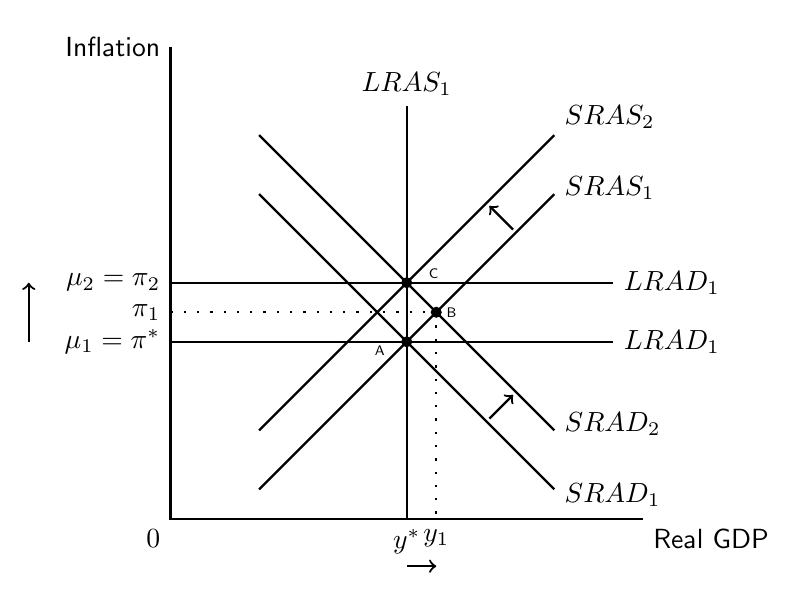
\begin{tikzpicture}[thick,font=\sffamily,scale=1.5]
	%axis
	\draw (0,4) node[left]{Inflation} -- (0,0) node[below left] {$0$} 
	  -- (4,0) node[below right]{Real GDP}; %labels
	%AS
	\draw[] (2,0) -- (2,3.5); %LRAS1	
	\draw plot[domain=0.75:3.25,smooth] (\x,-0.5+\x); %SRAS1
	\draw plot[domain=0.75:3.25,smooth] (\x,\x); %SRAS1
	
	%AD	 
	\draw[] (0,1.5) -- (3.75,1.5); %LRAD1
	\draw[] (0,2) -- (3.75,2); %LRAD2
	\draw plot[domain=0.75:3.25,smooth] (\x,3.5-\x); %SRAD1	 
	\draw plot[domain=0.75:3.25,smooth] (\x,4-\x); %SRAD1	
	 
	 %dotted lines
	 \draw[loosely dotted] (0,1.5) node[left]{$\mu_1=\pi^{*}$} -| node[pos=0.25,below=3mm] {}
	  (2,0) node[below]{$y^{*}$}; %dotted lines equib
	 \draw[loosely dotted] (0,1.75) node[left]{$\pi_1$} -| node[pos=0.25,below=3mm] {}
	  (2.25,0) node[below]{$y_1$}; %dotted lines shift
	 \draw[loosely dotted] (0,2) node[left]{$\mu_2=\pi_2$} -| node[pos=0.25,below=3mm] {}
	  (2,0) node[below]{}; %dotted lines new equib
	  

	
	%labels
	\node[above] at (2,3.5) {$LRAS_{1}$}; %LRAS1 label
	\node[right] at (3.75,1.5) {$LRAD_{1}$}; %LRAD1 label
	\node[right] at (3.75,2) {$LRAD_{1}$}; %LRAD2 label
	\node[right] at (3.25,2.8) {$SRAS_{1}$}; %SRAS1 label
	\node[right] at (3.25,3.4) {$SRAS_{2}$}; %SRAS2 label
	\node[right] at (3.25,0.2) {$SRAD_{1}$}; %SRAD1 label
	\node[right] at (3.25,0.8) {$SRAD_{2}$}; %SRAD2 label
	
	%arrows
	\draw [->] (2,-0.4) -- (2.25,-0.4); %x arrow
	\draw [->] (-1.2,1.5) -- (-1.2,2); %y arrow
	\draw [->] (2.7,0.85) -- (2.9,1.05); %SRAD arrow
	\draw [->] (2.9,2.45) -- (2.7,2.65); %SRAS arrow
	
	%dots
	\node[style={fill=black,circle,inner sep=0pt,minimum size=4pt}] at (2,1.5) { };equib
	\node[below left]at (1.9,1.55) {\tiny{A}};
	\node[style={fill=black,circle,inner sep=0pt,minimum size=4pt}] at (2.25,1.75) { };SR equib
	\node[right]at (2.25,1.75) {\tiny{B}};
	\node[style={fill=black,circle,inner sep=0pt,minimum size=4pt}] at (2,2) { };new LR equib
	\node[above right]at (2.1,1.95) {\tiny{C}};
	
\end{tikzpicture}
\end{document}
    \caption{The effect of a demand shock on an open macroeconomy in the short and long run}
    \label{fig:1}
\end{figure}
\begin{figure}[H]
    \centering
    \documentclass[class=article, crop=false]{standalone}
\usepackage{my_preamble}
\begin{document}
\begin{tikzpicture}[thick,font=\sffamily,scale=1.5]
 \draw (0,3.5) node[left]{$y=Y/L$} -- (0,0) node[below left] {$0$} 
  -- (6,0) node[below right]{$k=K/L$}; %labels
\draw [thick, name path = F1] (0,0) to [out=75,in=180] (5.5,3.2); %Production function
\draw [thick, name path = F1] (0,0) to (5.5,2.5); %R (cost)
\draw [dotted, name path = F1] (0,1.6) to (5.5,4.1); %Tangency with PF line

 \draw[loosely dotted] (0,2.6) node[left]{$y^{*}$} -| node[pos=0.25,below=3mm] {}
  (2.3,0) node[below]{$k^{*}$}; %optimum dotted lines

\node[right] at (5.5,3.2) {$y=f
(k)$}; %Production function label
%\node[right] at (5.5,1.8) {$S=s*f(k)$}; %Savings function label
\node[right] at (5.5,2.5) {$R=(1+r)*k$}; %Depreciation line label
%\draw [->] (1.85,-0.4) -- (1.25,-0.4); %x arrow
\end{tikzpicture}
\end{document}
    \caption{Neoclassical optimal level of capital per capita}
    \label{fig:2}
\end{figure}
\begin{figure}[ht]
	\begin{subfigure}{\textwidth}
		\centering
		\documentclass[class=article, crop=false]{standalone}
\usepackage{my_preamble}
\begin{document}
\begin{tikzpicture}[thick,font=\sffamily,scale=1.5]
 \draw (0,3.5) node[left]{$y=Y/L$} -- (0,0) node[below left] {$0$} 
  -- (6,0) node[below right]{$k=K/L$}; %labels
\draw [thick, name path = F1] (0,0) to [out=75,in=180] (5.5,3.2); %Production function
\draw [thick, name path = F1] (0,0) to (5.5,2.5); %R (cost)
\draw [dotted, name path = F1] (0,1.6) to (5.5,4.1); %Tangency with PF line

 \draw[loosely dotted] (0,2.6) node[left]{$y^{*}$} -| node[pos=0.25,below=3mm] {}
  (2.3,0) node[below]{$k^{*}$}; %optimum dotted lines

\node[right] at (5.5,3.2) {$y=f
(k)$}; %Production function label
%\node[right] at (5.5,1.8) {$S=s*f(k)$}; %Savings function label
\node[right] at (5.5,2.5) {$R=(1+r)*k$}; %Depreciation line label
%\draw [->] (1.85,-0.4) -- (1.25,-0.4); %x arrow
\end{tikzpicture}
\end{document} 
	\end{subfigure}
	\begin{subfigure}{\textwidth}
		\centering
		\documentclass[class=article, crop=false]{standalone}
\usepackage{my_preamble}
\begin{document}
\begin{tikzpicture}[thick,font=\sffamily,scale=1.5]
	%axis
	\draw (0,3.5) node[left]{$MPK$} -- (0,0) node[below left] {$0$} -- (6,0) node[below right]{$k=K/L$}; %labels
	
	%graphs
	\draw [thick, name path = F1] (0,2) to (5.5,2); %interest rate
	\draw [name path = F1] (0.5,3) to (5.3,0.3); %MPK line
	
	%dotted lines
	\draw[loosely dotted] (0,2) node[left]{$1+r$} -| node[pos=0.25,below=3mm] {}
	  (2.3,0) node[below]{$k^{*}$}; %optimum dotted lines
	%\draw[loosely dotted] (2.3,3.5) node[left]{} -| node[pos=0.25,below=3mm] {} (2.3,2) node[below]{}; %dotted line upwards
	
	%labels
	\node[right] at (3,2.3) {Marginal cost of capital$=(1+r)$}; %Savings function label
	\node[right] at (5.3,0.3) {$MPK$}; %MPK label
\end{tikzpicture}
\end{document}  
	\end{subfigure}
	\caption{The Neoclassical theory of investment, investing up to the point where $MPK=1+R$, where profits are maximised.}
	\label{fig:3}
\end{figure}
\begin{figure}[H]
    \centering
    \documentclass[class=article, crop=false]{standalone}
\usepackage{my_preamble}
\begin{document}
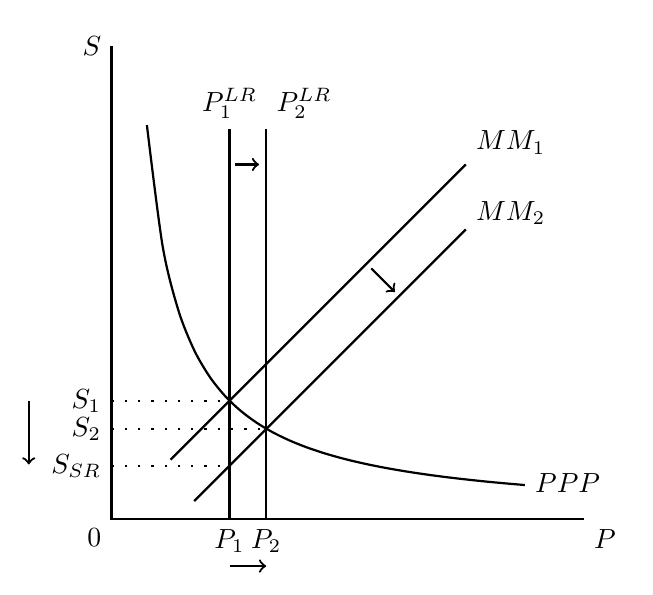
\begin{tikzpicture}[thick,font=\sffamily,scale=1.5]
	%axis and labels
	 \draw (0,4) node[left]{$S$} -- (0,0) node[below left] {$0$} 
	  -- (4,0) node[below right]{$P$};
	  
	%graphs
	\draw plot[domain=0.5:3,smooth] (\x,\x); %MM1
	\draw plot[domain=0.7:3,smooth] (\x,\x-0.55); %MM2
	\draw plot[domain=0.3:3.5,smooth] (\x,1/\x); %PPP1
	\draw[] (1,0) -- (1,3.3); %LR prices 1
	\draw[] (1.31,0) -- (1.31,3.3); %LR prices 2

	%labels
	\node[right] at (3.5,0.3) {$PPP$}; %PPP label
	\node[above] at (1,3.3) {$P^{LR}_1$}; %MM label  
	\node[above right] at (1.31,3.3) {$P^{LR}_2$}; %MM2 label  
	\node[above right] at (3,3) {$MM_{1}$}; %LR prices label 
	\node[above right] at (3,2.4) {$MM_{2}$}; %LR prices 2 label 
	
	%dotted lines
	\draw[loosely dotted] (0,1) node[left]{$S_1$} -| node[pos=0.25,below=3mm] {} (1,0) node[below]{$P_1$}; %S1 and P1
	\draw[loosely dotted] (0,0.76) node[left]{$S_2$} -| node[pos=0.25,below=3mm] {} (1.31,0) node[below]{$P_2$}; %S2 and P2
	\draw[loosely dotted] (0,0.45) node[left]{$S_{SR}$} -| node[pos=0.25,below=3mm] {} (1,0) node[below]{}; %x3 and horizontal lines
    
	%arrows
	\draw [->] (1,-0.4) -- (1.31,-0.4); %x arrow
	\draw [->] (-0.7,1) -- (-0.7,0.46); %y arrow
	\draw [->] (1.05,3) -- (1.25,3); %LR prices arrow
	\draw [->] (2.2,2.12) -- (2.4,1.92); %MM arrow

%---------------------------------------------------------------
%ALTERNATIVE GRAPHS	
	%\draw [thick, name path = F1] (0.2,3.5) to [out=270,in=180] (3.5,0.2); %PPP
	%\draw[] (1.15,0) -- (1.15,3); %LR prices
	
\end{tikzpicture}
\end{document}
    \caption{The effect of an increase in the nominal money stock in the Overshooting Model}
    \label{fig:4}
\end{figure}
\begin{figure}[H]
    \centering
    \documentclass[class=article, crop=false]{standalone}
\usepackage{my_preamble}
\begin{document}
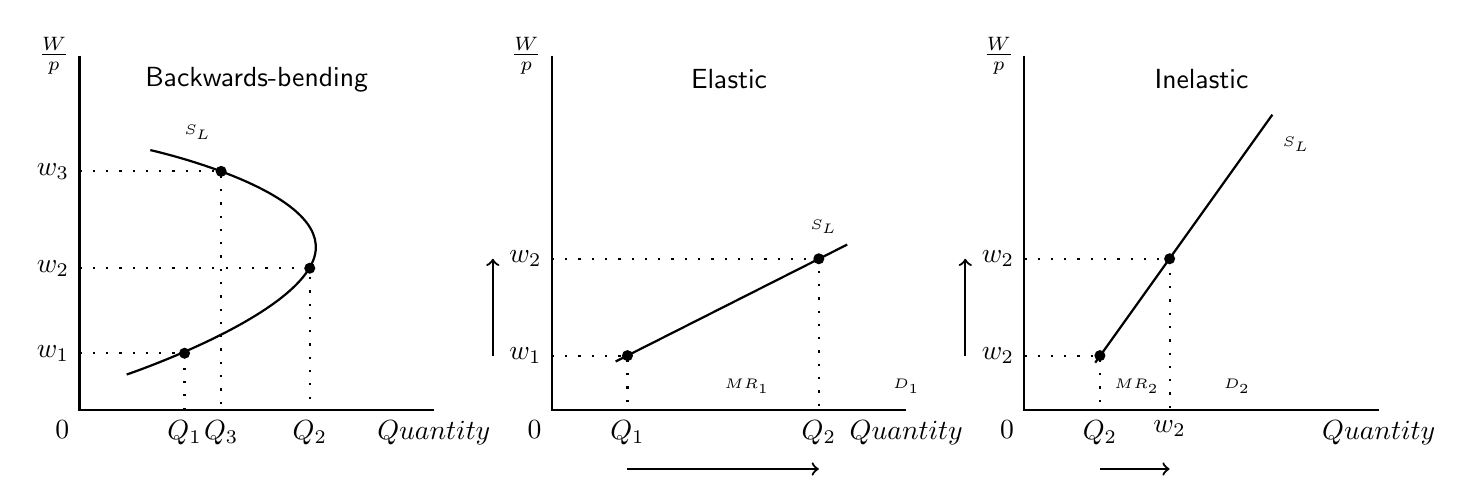
\begin{tikzpicture}[thick,font=\sffamily,scale=1.5]
	%axies
	\draw (-6,3) node[left]{$\frac{W}{p}$} -- (-6,0) node[below left] {$0$} -- (-3,0) node[below]{$Quantity$}; %market
	\draw (-2,3) node[left]{$\frac{W}{p}$} -- (-2,0) node[below left] {$0$} -- (1,0) node[below]{$Quantity$}; %type 1
	\draw (2,3) node[left]{$\frac{W}{p}$} -- (2,0) node[below left] {$0$} -- (5,0) node[below]{$Quantity$}; %type 2
	
	%titles
	\node[] at (-4.5,2.8) {Backwards-bending}; %Market title
	\node[] at (-0.5,2.8) {Elastic}; %Type 1 title
	\node[] at (3.5,2.8) {Inelastic}; %Market title
	  
	 %Backwards-bending D----------------------------------------------
	\node[right] at (-5.2,2.35) {\tiny{$S_{L}$}}; %Labour Supply label
	\draw[] plot [smooth, tension=1] coordinates {(-5.6,0.3) (-4,1.35) (-5.4,2.2)}; %Labour Supply
		%wage 1
		\node[style={fill=black,circle,inner sep=0pt,minimum size=4pt}] at (-5.11,0.48) { }; %node 1
		\draw[loosely dotted] (-6,0.48) node[left]{$w_{1}$} -| node[pos=0.25,below=3mm] {} (-5.11,0) node[below]{$Q_{1}$}; %dotted lines 1
		
		%wage 2
		\node[style={fill=black,circle,inner sep=0pt,minimum size=4pt}] at (-4.05,1.2) { }; %node 2
		\draw[loosely dotted] (-6,1.2) node[left]{$w_{2}$} -| node[pos=0.25,below=3mm] {} (-4.05,0) node[below]{$Q_{2}$}; %dotted lines 2
		
		%wage 3
		\node[style={fill=black,circle,inner sep=0pt,minimum size=4pt}] at (-4.8,2.02) { }; %node 3
		\draw[loosely dotted] (-6,2.02) node[left]{$w_{3}$} -| node[pos=0.25,below=3mm] {} (-4.8,0) node[below]{$Q_{3}$}; %dotted lines 3
	
	
	%Type 1 - elastic-------------------------------------
	\draw[] (-1.46,0.41) -- (0.5,1.4); %Elastic labour supply
	\node[right] at (0.1,1.55) {\tiny{$S_{L}$}}; %Labour Supply label
	\node[] at (1,0.2) {\tiny{$D_{1}$}}; %Demand1 label
	\node[] at (-0.35,0.2) {\tiny{$MR_{1}$}}; %MR1 label
	\node[style={fill=black,circle,inner sep=0pt,minimum size=4pt}] at (-1.36,0.46) { }; %mc=mr node
	\draw[loosely dotted] (-2,0.46) node[left]{$w_{1}$} -| node[pos=0.25,below=3mm] {} (-1.36,0) node[below]{$Q_{1}$}; %dotted lines
	
		%second wage
		\node[style={fill=black,circle,inner sep=0pt,minimum size=4pt}] at (0.26,1.28) { }; %node 2
		\draw[loosely dotted] (-2,1.28) node[left]{$w_{2}$} -| node[pos=0.25,below=3mm] {} (0.26,0) node[below]{$Q_{2}$}; %dotted lines 2
		
		%arrows
		\draw [->] (-1.36,-0.5) -- (0.26,-0.5); %x arrow
		\draw [->] (-2.5,0.46) -- (-2.5,1.28); %y arrow

	 
	%Type 2 - inelastic-----------------------------------
	\draw[] (2.6,0.4) -- (4.1,2.5); %Elastic labour supply
	\node[right] at (4.1,2.25) {\tiny{$S_{L}$}}; %Labour Supply label
	\node[] at (3.8,0.2) {\tiny{$D_{2}$}}; %Demand2 label
	\node[] at (2.95,0.2) {\tiny{$MR_{2}$}}; %MR2 label
	\node[style={fill=black,circle,inner sep=0pt,minimum size=4pt}] at (2.64,0.46) { }; %mc=mr node
	\draw[loosely dotted] (2,0.46) node[left]{$w_{2}$} -| node[pos=0.25,below=3mm] {} (2.64,0) node[below]{$Q_{2}$}; %dotted lines
	
		%second wage
		\node[style={fill=black,circle,inner sep=0pt,minimum size=4pt}] at (3.23,1.28) { }; %node 2
		\draw[loosely dotted] (2,1.28) node[left]{$w_{2}$} -| node[pos=0.25,below=3mm] {} (3.23,0) node[below]{$w_{2}$}; %dotted lines 2
		
		%arrows
		\draw [->] (2.64,-0.5) -- (3.23,-0.5); %x arrow
		\draw [->] (1.5,0.46) -- (1.5,1.28); %y arrow
		
\end{tikzpicture}
\end{document}
    \caption{The labour propagation mechanism of the Real Business Cycle model}
    \label{fig:5}
\end{figure}
\begin{figure}[H]
    \centering
    \documentclass[class=article, crop=false]{standalone}
\usepackage{my_preamble}
\begin{document}
\begin{tikzpicture}[thick,font=\sffamily,scale=1.5]
	%axis
	\draw (0,3.5) node[left]{$y=Y/L$} -- (0,0) node[below left] {$0$} -- (6,0) node[below right]{$k=K/L$}; %labels

	%graphs	
	\draw [thick, name path = F1] (0,0) to [out=75,in=180] (5.5,3.2); %Production function
	\draw [thick, name path = F1] (0,0) to [out=55,in=180] (5.5,1.8); %Savings function
	\draw [thick, name path = F1] (0,0) to (5.5,2.5); %Depreciation/Pop/TFP growth
	
	%dotted lines
	\draw [dotted, name path = F1] (0,1.6) to (5.5,4.1); %Tangency with PF line
	\draw[loosely dotted] (0,1.8) node[left]{$\bar{y}$} -| node[pos=0.25,below=3mm] {} (3.9,0) node[below]{$\bar{k}$}; %steady state dotted lines
	\draw[loosely dotted] (0,2.6) node[left]{$y^{*}$} -| node[pos=0.25,below=3mm] {} (2.3,0) node[below]{$k^{*}$}; %optimum dotted lines
  
	%labels
	\node[right] at (5.5,3.2) {$y=f(k)$}; %Production function label
	\node[right] at (5.5,1.8) {$saving=s*f(k)$}; %Savings function label
	\node[right] at (5.5,2.5) {$(\delta+\alpha + n)*k$}; %Depreciation line label
\end{tikzpicture}
\end{document}
    \caption{Steady state and the Golden Rule in the Solow model}
    \label{fig:6}
\end{figure}
\end{document}
